\chapter{模型视图教程}

每个 \hl{UI} 开发人员都应该了解模型视图编程,本教程的目的是让您轻松理解有关模型视图的相关知识。

表格,列表和树部件是 GUI 中经常使用的组件。这些部件可以通过两种不同的方式访问其数据。
传统方式是,这些部件包含用于存储数据的内部容器。这种方法非常直观,但是,在许多应用程序中,它会导致数据同步问题。
第二种方法是模型/视图编程,其中部件不维护内部数据容器。他们通过标准化接口访问外部数据,因此避免了数据重复。
乍一看,这似乎很复杂,但是如果您仔细看一看,不仅容易掌握,而且模型/视图编程的许多好处也变得更加明显。

\begin{figure}[hbt!]  
	% \centering
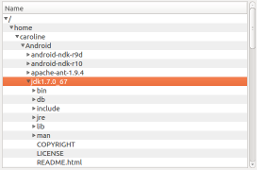
\includegraphics[width=0.3\textwidth]{treeview}
\end{figure}

在此过程中,我们将了解 \hl{Qt} 提供的一些基本技术,例如:

\begin{compactitem}
\item 标准部件和模型视图部件的区别
\item 窗体和模型之间的适配器
\item 开发一个简单的模型视图的应用程序
\item 预定义模型

\end{compactitem}

中间主题,比如

\begin{compactitem}
\item 树形视图
\item 选项
\item 委托
\item 模型调试测试
\end{compactitem}

您还将了解到新的应用程序是否可以通过模型/视图编程更容易地编写,或者经典的标准部件是否也可以工作。

本教程中的代码您可以编辑修改或者集成到您的项目中去。 源码在 \hl{Qt} 的 \hl{examples/widgets/tutorials/modelview} 目录。

详见 参考文档

\section{介绍}

模型/视图是一种将数据从视图中分离出来,来处理数据集的一种技术。标准部件并不是为将数据从视图中分离出来而设计的,这就是为什么 Qt 会有两种不同类型的部件。
这两种部件看起来都一样,但是它们与数据之间的交互方式是不同的。

\begin{tabular}{|l|m{25em}|}
	\hline
		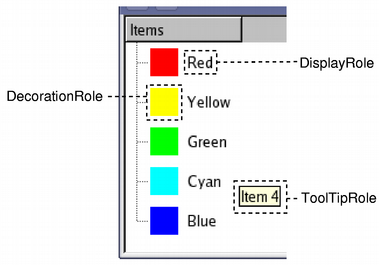
\includegraphics[width=0.5\textwidth]{modelview-roles}
	  & 
	项角色
	
	项角色向模型指示要引用的数据类型。视图可以以不同的方式显示角色,因此为每个角色提供适当的信息很重要。
	
	创建新模型 部分将更详细地介绍角色的某些特定用法。\\
	\hline	
	\end{tabular}